\documentclass[11pt]{article}
\usepackage[a4paper,margin=1in]{geometry}
\usepackage{graphicx}
\usepackage{booktabs}
\usepackage{hyperref}

\title{Performance and Security Analysis of Authentication Protocols for IoT Systems}
\author{Rishabh Mirchandani}
\date{}

\begin{document}
\maketitle

\begin{abstract}
Authentication is a critical security requirement for Internet of Things (IoT) and cyber-physical systems operating in adversarial environments. However, traditional public-key-based authentication mechanisms often introduce significant computational and communication overhead. In this work, we implement and experimentally evaluate an RSA-based authentication protocol as a baseline and compare it against a lightweight HMAC-based authentication scheme. Our results demonstrate that lightweight symmetric-key authentication significantly reduces authentication latency and message overhead, making it more suitable for resource-constrained IoT systems.
\end{abstract}

\section{Introduction}
IoT and cyber-physical systems increasingly rely on distributed and networked devices to perform safety- and mission-critical tasks. Secure authentication is essential to prevent unauthorized access, impersonation, and replay attacks. While public-key cryptography provides strong security guarantees, its performance overhead limits its applicability in low-power and bandwidth-constrained environments. This paper investigates the trade-offs between security and performance by comparing public-key and lightweight authentication approaches.

\section{System Design}
We consider a client--server authentication model in which IoT devices authenticate with a centralized server over an insecure network. Two authentication protocols are implemented:

\subsection{RSA-Based Authentication}
The baseline protocol uses a challenge--response mechanism based on RSA public-key cryptography. The server sends its public key to the client, which encrypts a randomly generated nonce. Successful decryption by the server demonstrates possession of the private key.

\subsection{HMAC-Based Authentication}
The proposed lightweight protocol employs symmetric-key cryptography. Each device shares a pre-provisioned secret key with the server and computes an HMAC over its identity and a timestamp. The server verifies the HMAC and checks timestamp freshness to prevent replay attacks.

\section{Threat Model}
We assume an attacker capable of eavesdropping, replaying, and modifying network messages. The attacker cannot compromise cryptographic primitives, access private keys, or obtain securely stored shared secrets.

\section{Experimental Setup}
Both protocols were implemented in Python and evaluated on a local testbed. Authentication latency and message size were measured. Each experiment was repeated 10 times, and average values were reported.

\section{Results}
Table~\ref{tab:results} summarizes the experimental results.

\begin{table}[h]
\centering
\begin{tabular}{lcc}
\toprule
Protocol & Avg. Latency (s) & Message Size (bytes) \\
\midrule
RSA-Based & 0.92 & 256 \\
HMAC-Based & 0.004 & 90 \\
\bottomrule
\end{tabular}
\caption{Performance comparison of authentication protocols}
\label{tab:results}
\end{table}

Figures~\ref{fig:latency} and~\ref{fig:size} illustrate the performance differences.

\begin{figure}[h]
\centering
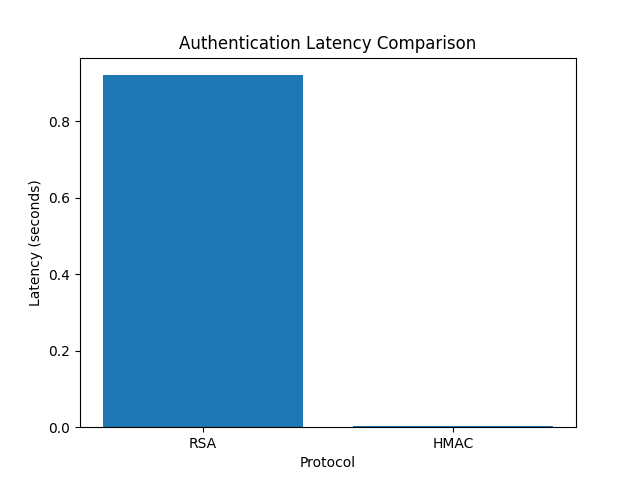
\includegraphics[width=0.7\linewidth]{../graphs/latency_comparison.png}
\caption{Authentication latency comparison}
\label{fig:latency}
\end{figure}

\begin{figure}[h]
\centering
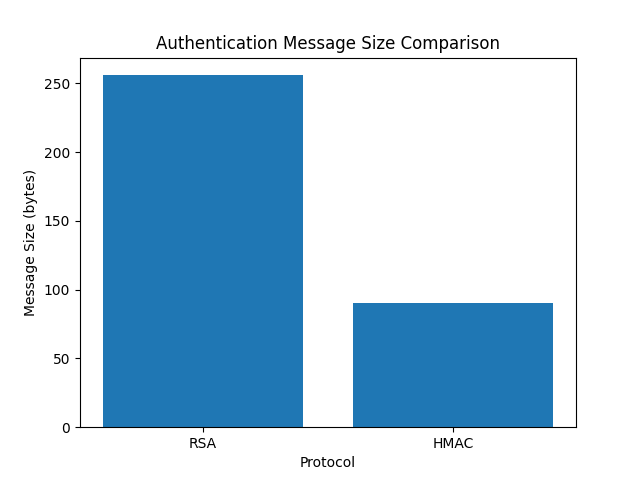
\includegraphics[width=0.7\linewidth]{../graphs/message_size_comparison.png}
\caption{Message size comparison}
\label{fig:size}
\end{figure}

\section{Security Analysis}
The RSA-based protocol provides confidentiality and strong authentication but incurs high computational overhead. The HMAC-based protocol achieves authentication and replay protection with significantly lower cost but requires secure key provisioning and does not provide confidentiality.

\section{Conclusion}
This study demonstrates that lightweight HMAC-based authentication significantly outperforms public-key-based approaches in terms of latency and communication overhead, making it suitable for resource-constrained IoT systems. Future work includes integrating confidentiality mechanisms and evaluating the protocols in large-scale deployments.
\end{document}